% ─────────────────────────────────────────────────────────────────────────────
% APÉNDICE B — Marco de Criterios, Métricas y Modelo de Decisión CNI (OE3)
% ─────────────────────────────────────────────────────────────────────────────

% ── Paleta de colores del apéndice ──────────────────────────────────────────
\definecolor{oe3azul}    {HTML}{1A3F6F}   % encabezados principales
\definecolor{oe3azulcl}  {HTML}{E8EEF7}   % filas alternas
\definecolor{oe3verde}   {HTML}{1B5E20}   % Excelente
\definecolor{oe3verdecl} {HTML}{E8F5E9}
\definecolor{oe3ambar}   {HTML}{E65100}   % Aceptable
\definecolor{oe3ambarcl} {HTML}{FFF3E0}
\definecolor{oe3rojo}    {HTML}{B71C1C}   % Deficiente
\definecolor{oe3rojocl}  {HTML}{FFEBEE}
\definecolor{oe3gris}    {HTML}{546E7A}   % subtítulos
\definecolor{oe3griscl}  {HTML}{F5F5F5}  % fondo de notas

\newcolumntype{Z}{>{\centering\arraybackslash}X}

\chapter{Marco de Criterios y Modelo de Decisión CNI} \label{chap:apendice_oe3}

\section{Introducción y el dilema de la selección de CNI} \label{sec:apb_intro}

En la arquitectura de Kubernetes, el plano de datos depende del \emph{Container Network Interface} (CNI). Al no existir un plugin de red por defecto, la elección recae sobre los ingenieros de infraestructura, quienes a menudo deciden por popularidad o guías rápidas, omitiendo un análisis cuantitativo sistemático de rendimiento.

El reto principal de elegir un CNI es que no existe una única solución óptima en todas las dimensiones simultáneamente. El rendimiento base de velocidad de red (\emph{throughput}) es solo una dimensión del problema. Por ejemplo, una pasarela de transacciones bancarias exige seguridad estricta y aislamiento lógico, mientras que un clúster IoT en nodos con recursos de cómputo limitados prioriza un bajo consumo de memoria RAM y CPU.

La Tabla~\ref{tab:apb_tradeoffs} muestra a nivel conceptual este compromiso de rendimiento (\emph{trade-off}) cualitativo entre los plugins evaluados, sirviendo de introducción visual al dilema de selección.

\begin{table}[htbp]
\centering
\scriptsize
\caption{Matriz comparativa cualitativa de compromisos (trade-offs) en CNIs.}
\label{tab:apb_tradeoffs}
\begin{tabularx}{\textwidth}{|Y|c|c|c|c|}
\hline
\textbf{Dimensión} & \textbf{Flannel} & \textbf{Calico} & \textbf{Cilium} & \textbf{Antrea} \\
\hline
Latencia y jitter & Medio & Excelente & Bueno & Aceptable \\
Throughput & Bueno & Excelente & Aceptable & Bueno \\
Consumo de CPU & Excelente & Deficiente & Aceptable & Aceptable \\
Consumo de RAM & Excelente & Deficiente & Aceptable & Aceptable \\
Network Policies L4 & Nulo (No soporta) & Excelente & Excelente & Excelente \\
Network Policies L7 & Nulo (No soporta) & Nulo (No soporta) & Excelente & Nulo (No soporta) \\
\hline
\end{tabularx}
\end{table}

Para dar solución a este problema de forma cuantitativa, este apéndice documenta el desarrollo y validación del Objetivo Específico 3 de la tesis: un modelo formal compuesto por criterios jerárquicos, métricas normalizadas, umbrales de calidad de servicio (SLA) y ponderaciones específicas de negocio.

% ─────────────────────────────────────────────────────────────────────────────
\section{Definición de criterios y métricas de evaluación} \label{sec:apb_criterios}

Para comparar los plugins de manera objetiva, el modelo agrupa los indicadores en tres criterios principales (C1, C2 y C3), resumidos en la Tabla~\ref{tab:apb_criterios}.

\begin{table}[htbp]
\centering
\scriptsize
\caption{Estructura de criterios, preguntas de control y métricas del modelo de selección.}
\label{tab:apb_criterios}
\begin{tabularx}{\textwidth}{|l|l|Y|}
\hline
\textbf{Criterio Principal} & \textbf{Pregunta de Control (UI)} & \textbf{Métricas y Variables Asociadas} \\
\hline
\textbf{C1: Rendimiento de Red (QoS)} & ¿Qué tan rápido tiene que responder? & Latencia base promedio (ms), Latencia máxima (ms) \\
\cline{2-3}
& ¿Qué tan estable debe ser la conexión? & Jitter (MDEV) (ms), Retransmisiones TCP (paquetes/sesión) \\
\cline{2-3}
& ¿Cuántos datos se van a mover al mismo tiempo? & Throughput TCP promedio (Mbps) \\
\hline
\textbf{C2: Eficiencia de Recursos} & ¿Los servidores donde va a funcionar son pequeños? & Consumo de CPU promedio (\% del nodo), Consumo de RAM promedio (MB) \\
\hline
\textbf{C3: Impacto de Seguridad} & ¿Qué tan importante es la seguridad y el control? & Soporte nativo de Network Policies, Sobrecarga (overhead) de latencia y throughput (\%) \\
\hline
\end{tabularx}
\end{table}

\begin{itemize}
  \item \textbf{C1 --- Rendimiento de red (QoS):} Evalúa latencia promedio/máxima, inestabilidad (\emph{jitter}), velocidad de transferencia (\emph{throughput}) y retransmisiones (pérdida de paquetes).
  \item \textbf{C2 --- Eficiencia de recursos:} Mide el consumo de CPU y memoria RAM que el agente CNI requiere en cada nodo worker para funcionar.
  \item \textbf{C3 --- Impacto de seguridad:} Mide la sobrecarga (\emph{overhead}) de latencia y throughput al activar Network Policies en el clúster.
\end{itemize}

% ─────────────────────────────────────────────────────────────────────────────
\section{Datos experimentales consolidados del testbed} \label{sec:apb_datos}

Para alimentar el modelo matemático de decisión, se recolectaron datos cuantitativos de las pruebas experimentales del testbed. Los detalles técnicos del clúster de laboratorio (número de nodos, tipo de recursos, configuración de red e infraestructura cloud en DigitalOcean) y la metodología de recolección ya han sido ampliamente descritos en los Capítulos 7 y 8 de este documento.

Tras aplicar el filtro estadístico de rango intercuartílico (IQR) para eliminar valores atípicos, se obtuvieron las medias consolidadas que sirven como entrada del modelo. La Tabla~\ref{tab:apb_datos_reales} presenta estos valores cuantitativos reales obtenidos del testbed.

\begin{table}[htbp]
\centering
\scriptsize
\caption{Resultados experimentales consolidados del testbed con indicadores de optimización.}
\label{tab:apb_datos_reales}
\begin{tabularx}{\textwidth}{|Y|c|c|c|c|}
\hline
\textbf{Métrica de Entrada} & \textbf{Flannel} & \textbf{Calico} & \textbf{Cilium} & \textbf{Antrea} \\
\hline
Latencia base promedio ($\downarrow$) & 21.53 ms & 12.54 ms & 18.73 ms & 35.09 ms \\
Latencia máxima ($\downarrow$) & 50.80 ms & 44.20 ms & 47.00 ms & 83.50 ms \\
Jitter (MDEV) ($\downarrow$) & 7.76 ms & 7.31 ms & 8.47 ms & 17.25 ms \\
Throughput TCP promedio ($\uparrow$) & 1452.97 Mbps & 1804.40 Mbps & 843.56 Mbps & 1588.45 Mbps \\
Retransmisiones TCP promedio ($\downarrow$) & 11774 paq. & 68993 paq. & 15142 paq. & 42229 paq. \\
CPU bajo estrés ($\downarrow$) & 19.45\% & 29.05\% & 25.79\% & 27.75\% \\
RAM bajo estrés ($\downarrow$) & 1176.54 MB & 1672.83 MB & 1497.19 MB & 1429.95 MB \\
\hline
\end{tabularx}
\end{table}

Para facilitar la interpretación de los datos, cada métrica incluye un indicador del sentido óptimo del valor:
\begin{itemize}
  \item \textbf{Sentido descendente $(\downarrow)$:} Indica que un valor menor representa un mejor comportamiento técnico. Por ejemplo, en la latencia base, el valor de Calico ($12,54$ ms) es superior al de Flannel ($21,53$ ms) porque reduce el retardo de transmisión. Lo mismo aplica para el jitter, consumo de CPU, RAM y retransmisiones TCP.
  \item \textbf{Sentido ascendente $(\uparrow)$:} Indica que un valor mayor representa un mejor comportamiento técnico. Se utiliza principalmente en el \emph{throughput} (ancho de banda disponible).
\end{itemize}

% ─────────────────────────────────────────────────────────────────────────────
\section{Normalización continua Min-Max} \label{sec:apb_umbrales}

Para estandarizar las métricas crudas y permitir la suma ponderada del modelo MCDA, el algoritmo procesador aplica una función de normalización \emph{min-max} continua que proyecta los valores a una escala uniforme de $1.00$ a $5.00$. A diferencia de los modelos basados en umbrales discretos escalonados, esta aproximación refleja proporcional y exactamente las brechas de rendimiento entre los plugins evaluados.

La Ecuación~\ref{eq:apb_minmax} define la transformación para las métricas donde un mayor valor es mejor (ej. \emph{throughput}), y la Ecuación~\ref{eq:apb_minmax_inv} se utiliza para aquellas métricas donde un menor valor es el deseable (ej. latencia, retransmisiones, consumo de CPU y RAM).

\begin{equation}
  V_{norm} = 1 + \left( \frac{V_{crudo} - Min}{Max - Min} \right) \times 4
  \label{eq:apb_minmax}
\end{equation}

\begin{equation}
  V_{norm} = 1 + \left( \frac{Max - V_{crudo}}{Max - Min} \right) \times 4
  \label{eq:apb_minmax_inv}
\end{equation}

Los resultados normalizados garantizan que el CNI con el mejor desempeño en una dimensión obtenga exactamente $5.00$ y el de peor desempeño obtenga exactamente $1.00$.

% ─────────────────────────────────────────────────────────────────────────────
\section{Factores de ponderación y restricciones no compensatorias} \label{sec:apb_ponderaciones}

El modelo aplica factores de ponderación (pesos porcentuales) que suman el $100\%$ ($1,0$), asignando mayor peso a las métricas más críticas según el caso de uso. La distribución de pesos calculados dinámicamente por la herramienta para los tres perfiles base se muestra en la Tabla~\ref{tab:apb_pesos}.

\begin{table}[htbp]
\centering
\scriptsize
\caption{Matriz de factores de ponderación (pesos calculados) por perfil de la tesis.}
\label{tab:apb_pesos}
\begin{tabularx}{\textwidth}{|Y|c|c|c|c|c|}
\hline
\textbf{Perfil / Caso de Uso} & \textbf{Latencia} & \textbf{Estabilidad} & \textbf{Throughput} & \textbf{Recursos} & \textbf{Seguridad} \\
\hline
Fintech / Seguridad crítica & 20.8\% & 24.8\% & 21.0\% & 8.1\% & 25.3\% \\
\hline
Streaming / Alto rendimiento & 27.7\% & 22.7\% & 25.1\% & 12.3\% & 12.3\% \\
\hline
IoT / Recursos limitados & 20.8\% & 19.0\% & 18.5\% & 28.0\% & 13.7\% \\
\hline
\end{tabularx}
\end{table}

\subsection{Restricción no compensatoria de seguridad}
Si se define un nivel de seguridad \emph{Alto} o \emph{Muy Alto} (como en el perfil Fintech), el modelo aplica una penalización directa al puntaje final de cualquier CNI que carezca de soporte nativo para Network Policies (como Flannel). Esto reduce su puntaje general al $40\%$ del valor ponderado calculado:

\begin{equation}
  P_{\text{final}} =
  \begin{cases}
    P_{\text{MCDA}} \times 0,40 & \text{si la seguridad es prioritaria y el CNI carece de políticas} \\
    P_{\text{MCDA}}               & \text{en caso normal}
  \end{cases}
  \label{eq:penalizacion_apb}
\end{equation}

Esta restricción matemática asegura que los plugins con falencias críticas en el plano de seguridad sean descartados automáticamente en entornos regulados, invalidando victorias engañosas logradas puramente mediante ventajas en la eficiencia de recursos computacionales.

% ─────────────────────────────────────────────────────────────────────────────
\section{Modelo matemático de decisión multicriterio (MCDA)} \label{sec:apb_mcda}

Para la recomendación formal del CNI, el algoritmo aplica el modelo MCDA de sumatoria ponderada clásica~\cite{ref34}:

\begin{equation}
  P_{\text{CNI}} = \sum_{i=1}^{n} V_i \times W_i
  \label{eq:mcda-formula}
\end{equation}

Donde $P_{\text{CNI}}$ es el puntaje del plugin para el perfil; $V_i$ es la puntuación normalizada (5, 3 o 1 punto) asignada según la métrica $i$ y sus umbrales; $W_i$ es el peso porcentual de la métrica en el perfil; y $n$ es el número de métricas evaluadas. 

La escala final de los puntajes del modelo MCDA está normalizada en la escala de $1,0$ a $5,0$, donde una puntuación de $5,0$ representa un CNI con comportamiento ideal (cumplimiento excelente de todos los requisitos prioritarios) y $1,0$ representa un cumplimiento totalmente deficiente del perfil evaluado.

El flujo de procesamiento del recomendador interactivo se resume a continuación:

\begin{center}
  \begin{tabular}{ccccccc}
    \colorbox{oe3azulcl}{\small\textbf{JSON/CSV crudos}} &
    $\rightarrow$ &
    \colorbox{oe3griscl}{\small\textbf{Filtro IQR}} &
    $\rightarrow$ &
    \colorbox{oe3griscl}{\small\textbf{Norm.\ min-max}} &
    $\rightarrow$ &
    \colorbox{oe3verdecl}{\small\textbf{$\sum V_i \times W_i$}} \\[6pt]
    \multicolumn{7}{c}{$\downarrow$} \\[4pt]
    \multicolumn{7}{c}{\colorbox{oe3azulcl}{\small\textbf{$P_{\text{CNI}}$: El CNI con la puntuación más alta es la recomendación del modelo}}}
  \end{tabular}
\end{center}

% ─────────────────────────────────────────────────────────────────────────────
\section{Resultados MCDA y análisis de selección} \label{sec:apb_resultados}

La Tabla~\ref{tab:apb_resultados} detalla las puntuaciones finales reales del análisis MCDA para cada plugin. El símbolo de asterisco ($*$) destaca la recomendación ganadora del modelo para cada perfil.

\begin{table}[htbp]
\centering
\scriptsize
\caption{Puntuaciones consolidadas del modelo MCDA reales para cada perfil (escala 1--5).}
\label{tab:apb_resultados}
\begin{tabularx}{\textwidth}{|Y|c|c|c|c|}
\hline
\textbf{Perfil de Usuario} & \textbf{Flannel} & \textbf{Calico} & \textbf{Cilium} & \textbf{Antrea} \\
\hline
Fintech / Seguridad crítica & 1.331 & 3.168 & * \textbf{3.631} & 2.211 \\
\hline
Streaming / Alto rendimiento & * \textbf{3.686} & 3.567 & 3.294 & 2.256 \\
\hline
IoT / Recursos limitados & * \textbf{3.834} & 2.952 & 3.232 & 2.224 \\
\hline
\end{tabularx}
\end{table}

\subsection{Interpretación y desglose de resultados}

\begin{itemize}
  \item \textbf{Perfil Fintech / Seguridad:} Cilium obtiene la puntuación óptima con $3.631$ (en la escala de 1 a 5). A pesar de que Calico ofrece un rendimiento crudo superior en latencia base, Cilium sobresale debido a sus políticas dinámicas de capa 7 basadas en eBPF~\cite{ref10} y su menor degradación del tráfico cuando el aislamiento lógico está activo.
  
  Por el contrario, Flannel obtiene un puntaje críticamente bajo de $1.331$. Esto se debe a que carece por diseño de soporte de Network Policies. Su puntuación base ponderada original de $3.328$ (impulsada principalmente por su bajo consumo de CPU y RAM) se somete a la penalización de seguridad de la Ecuación~\eqref{eq:penalizacion_apb}, multiplicándose por $0,4$. Esto demuestra cómo el modelo descarta automáticamente soluciones no aptas para entornos regulados.
  
  \textbf{Réplica en el Recomendador SPA:} Para obtener exactamente este resultado de $3.631$, el usuario debe establecer en el panel de control del recomendador las siguientes prioridades en los deslizadores (sliders):
  \begin{itemize}
    \item Latencia: \emph{Medio} ($3/5$)
    \item Estabilidad (Jitter): \emph{Muy Alto} ($5/5$)
    \item Throughput: \emph{Alto} ($4/5$)
    \item Límite de Recursos: \emph{Muy Bajo} ($1/5$)
    \item Nivel de Seguridad: \emph{Muy Alto} ($5/5$)
  \end{itemize}
  Esta selección genera ponderaciones específicas (Latencia $20.8\%$, Estabilidad $24.8\%$, Throughput $21.0\%$, Recursos $8.1\%$ y Seguridad $25.3\%$). Al requerirse un nivel de seguridad crítico, se activa automáticamente la penalización del factor $\times 0,40$ sobre Flannel. La configuración y los resultados se demuestran visualmente en la Figura~\ref{fig:rec_fintech_preguntas} (configuración de entrada) y la Figura~\ref{fig:rec_fintech_resultados} (salida final del prototipo web).

  \begin{figure}[htbp]
  \centering
  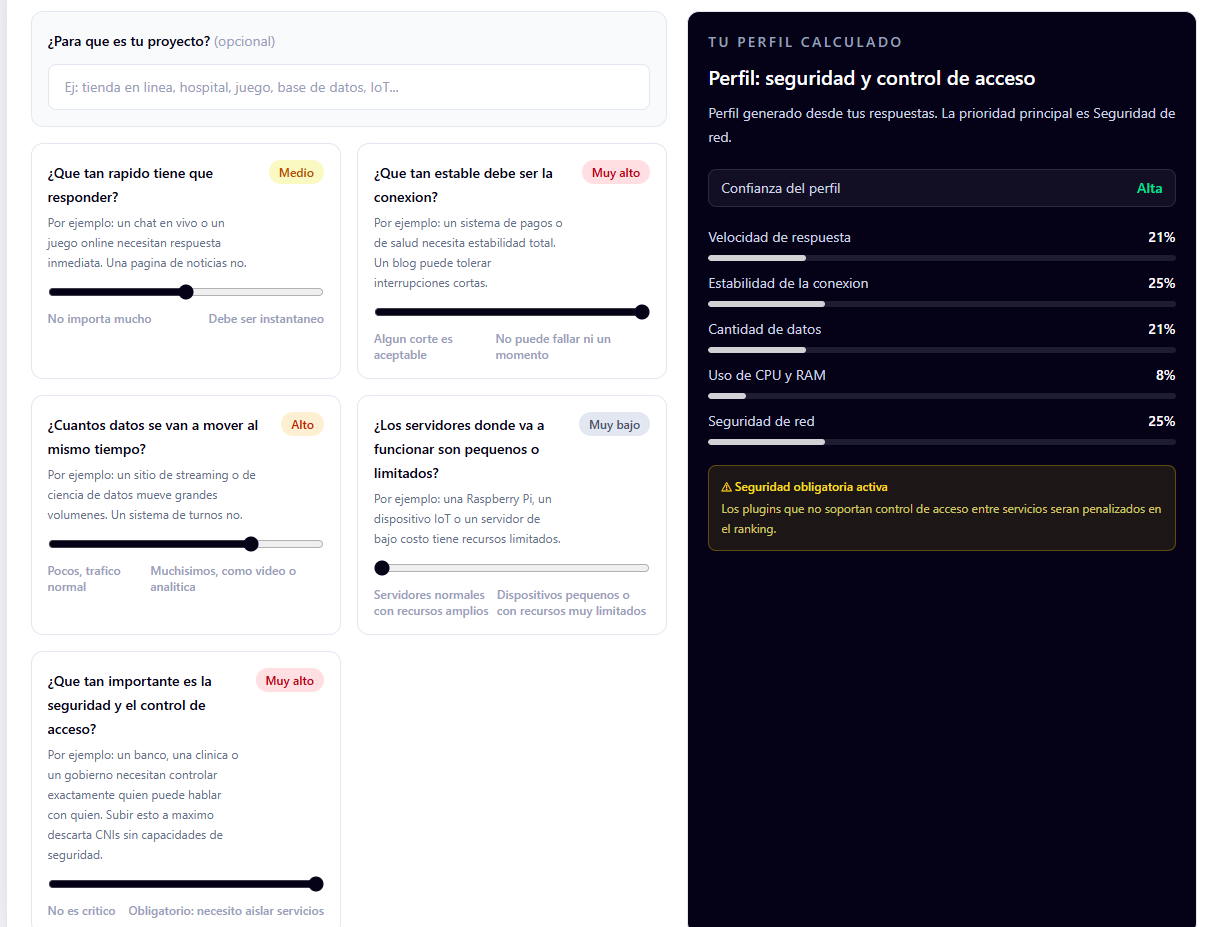
\includegraphics[width=0.85\textwidth]{figures/rec_fintech_preguntas.png}
  \caption{Configuración de sliders para el perfil Fintech / Seguridad en el Recomendador CNI.}
  \label{fig:rec_fintech_preguntas}
  \end{figure}

  \begin{figure}[htbp]
  \centering
  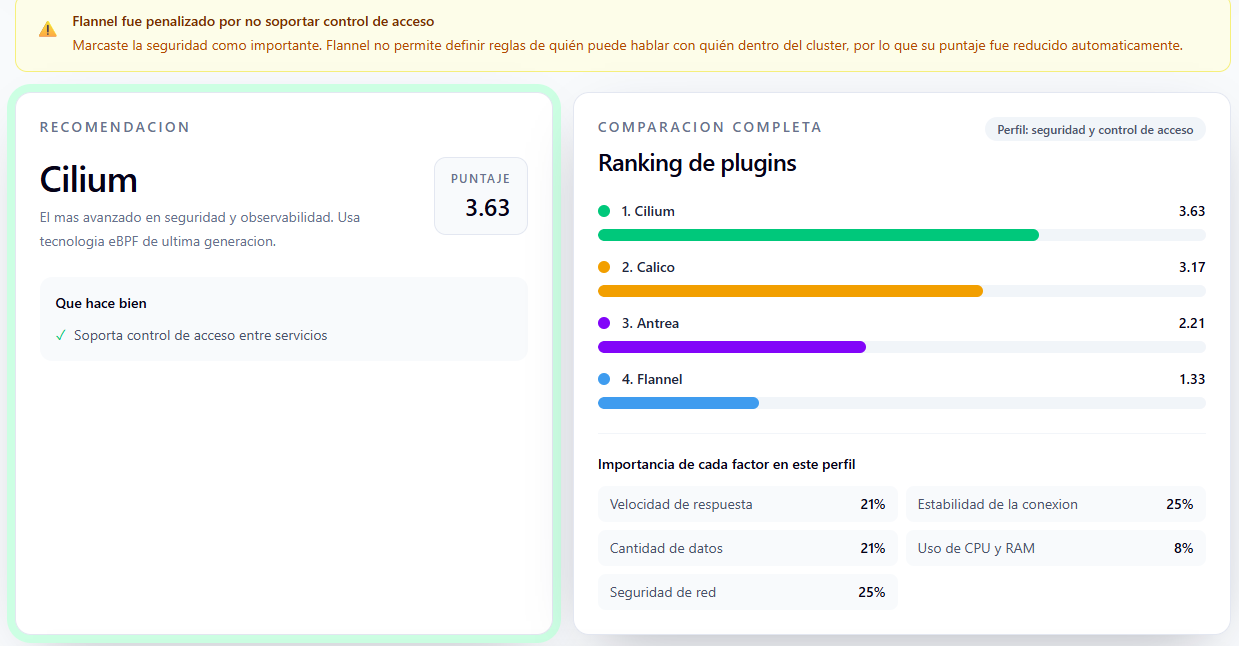
\includegraphics[width=0.95\textwidth]{figures/rec_fintech.png}
  \caption{Resultados del ranking MCDA en el prototipo interactivo para el perfil Fintech / Seguridad (Ganador: Cilium con 3.631).}
  \label{fig:rec_fintech_resultados}
  \end{figure}
  
  \item \textbf{Perfil Streaming / Rendimiento:} Flannel resulta recomendado con un puntaje de $3.686$. En el testbed, Flannel demostró un rendimiento balanceado y la estabilidad de red más alta al registrar solo 11,774 retransmisiones TCP frente a las 68,993 de Calico. Dado que la tasa de reenvío influye en la estabilidad de la transmisión de flujos continuos, la robustez de Flannel sumada a su eficiencia computacional compensa el mayor throughput bruto de Calico.
  
  \textbf{Réplica en el Recomendador SPA:} Para replicar el puntaje de $3.686$ de Flannel y $3.567$ de Calico, el usuario debe establecer las siguientes prioridades:
  \begin{itemize}
    \item Latencia: \emph{Muy Alto} ($5/5$)
    \item Estabilidad (Jitter): \emph{Alto} ($4/5$)
    \item Throughput: \emph{Muy Alto} ($5/5$)
    \item Límite de Recursos: \emph{Bajo} ($2/5$)
    \item Nivel de Seguridad: \emph{Bajo} ($2/5$)
  \end{itemize}
  Esta configuración prioriza la QoS de red cruda (throughput y latencia con pesos del $25.1\%$ y $27.7\%$ respectivamente) sin requerir seguridad restrictiva, lo que resulta en la victoria de Flannel por estabilidad.
  
  \item \textbf{Perfil IoT / Recursos limitados:} Flannel se posiciona como el CNI recomendado con $3.834$ frente a Cilium ($3.232$), Calico ($2.952$) y Antrea ($2.224$). Flannel destaca como el plugin que induce el menor estrés general bajo carga ($19.45\%$ de CPU del nodo y $1176.54$ MB de RAM global), lo cual se alinea con la prioridad de este perfil (28\% de peso a la eficiencia de recursos). Como se discute en el Capítulo~\ref{sec:Resultados}, esta métrica de RAM captura la huella del host bajo tráfico activo; un despliegue en nodos muy pequeños deberá aislar adicionalmente el consumo del binario en reposo.
  
  \textbf{Réplica en el Recomendador SPA:} Para replicar el puntaje de $3.834$ de Flannel, el usuario debe configurar los sliders con los siguientes valores:
  \begin{itemize}
    \item Latencia: \emph{Medio} ($3/5$)
    \item Estabilidad (Jitter): \emph{Medio} ($3/5$)
    \item Throughput: \emph{Medio} ($3/5$)
    \item Límite de Recursos: \emph{Muy Alto} ($5/5$)
    \item Nivel de Seguridad: \emph{Bajo} ($2/5$)
  \end{itemize}
  Esta selección asigna un $28.0\%$ de peso a la eficiencia de recursos. La Figura~\ref{fig:rec_iot_preguntas} y la Figura~\ref{fig:rec_iot_resultados} muestran respectivamente la entrada en la interfaz de usuario y el gráfico de barras resultante de la recomendación interactiva del sistema.

  \begin{figure}[htbp]
  \centering
  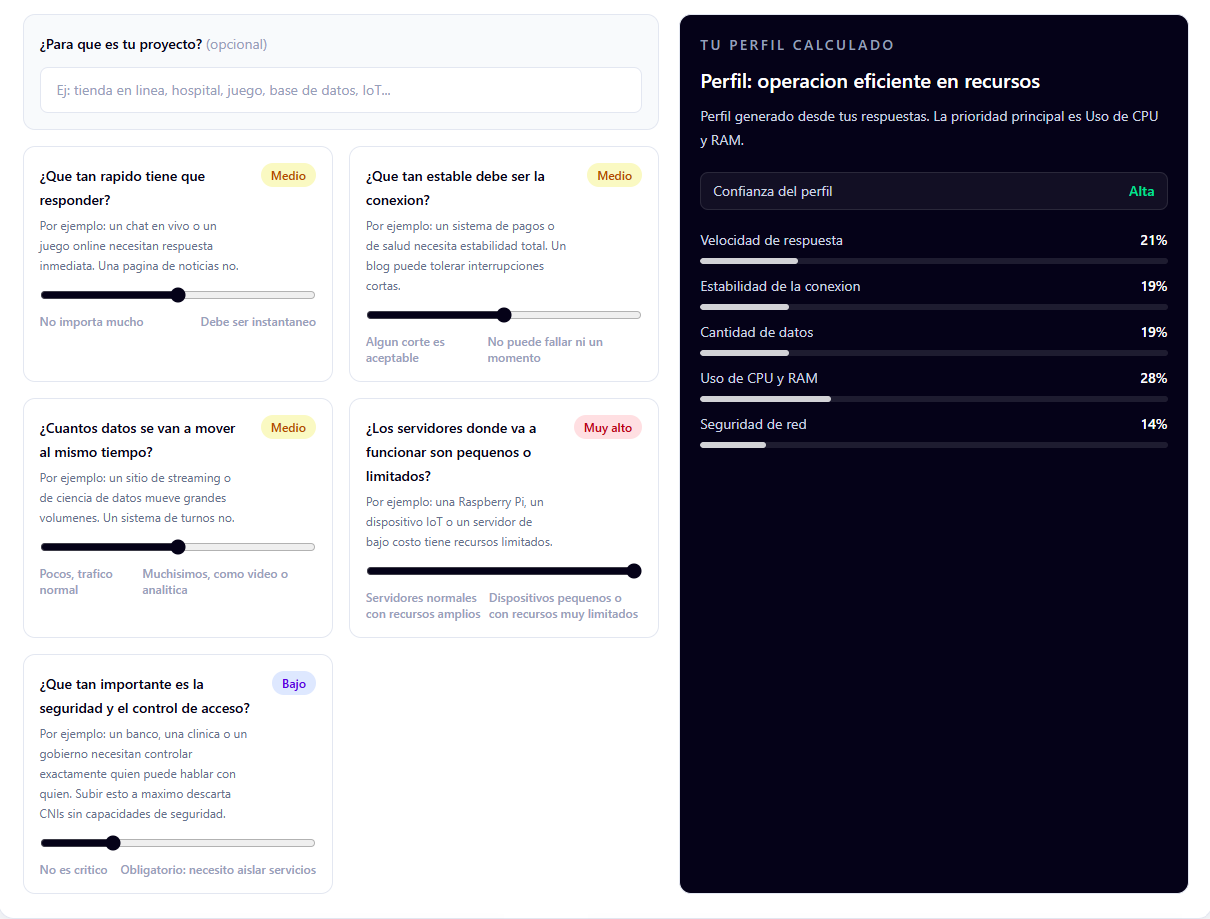
\includegraphics[width=0.85\textwidth]{figures/rec_iot_preguntas.png}
  \caption{Configuración de sliders para el perfil IoT / Recursos Limitados en el Recomendador CNI.}
  \label{fig:rec_iot_preguntas}
  \end{figure}

  \begin{figure}[htbp]
  \centering
  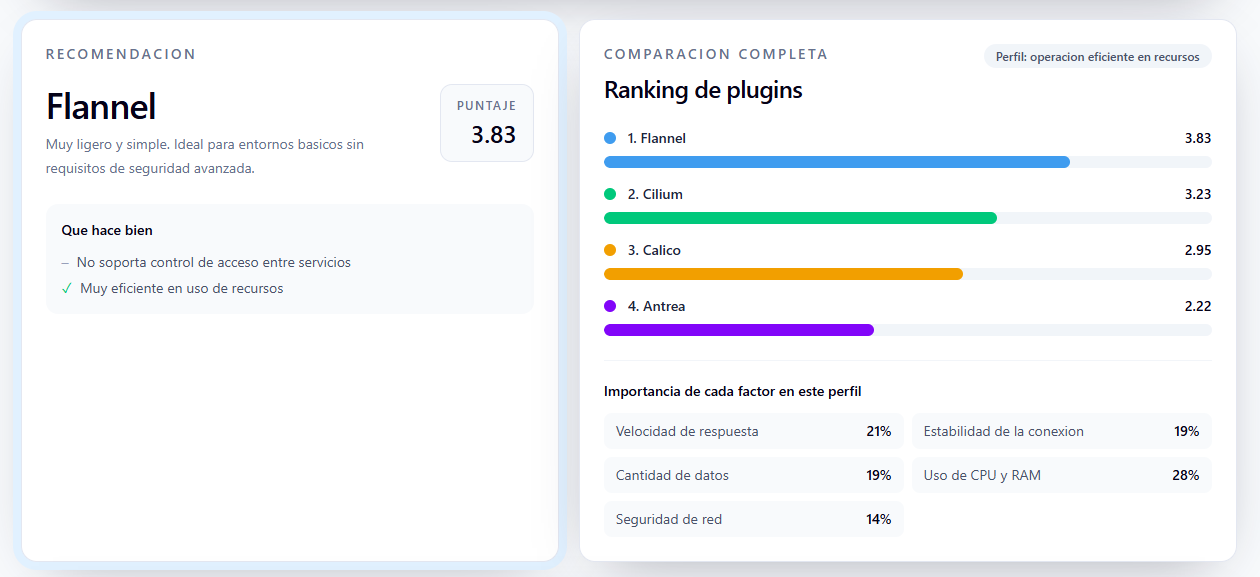
\includegraphics[width=0.95\textwidth]{figures/rec_iot.png}
  \caption{Resultados del ranking MCDA en el prototipo interactivo para el perfil IoT / Recursos Limitados (Ganador: Flannel con 3.834).}
  \label{fig:rec_iot_resultados}
  \end{figure}
\end{itemize}

\section{Lista de verificación para la configuración del recomendador CNI} \label{sec:apb_checklist}

El recomendador interactivo opera mediante cinco deslizadores de prioridad, cada uno en la escala \emph{Muy Bajo} (1) --- \emph{Bajo} (2) --- \emph{Medio} (3) --- \emph{Alto} (4) --- \emph{Muy Alto} (5). La combinación de valores genera los pesos porcentuales del modelo MCDA y, cuando la seguridad supera el nivel~4, activa la penalización no compensatoria $\times 0{,}40$ sobre plugins sin soporte de \texttt{NetworkPolicy}.

Esta lista de verificación es un instrumento cualitativo: mediante preguntas orientadas al contexto operativo del equipo, guía la asignación de cada deslizador antes de acceder al recomendador. No requiere mediciones previas; basta con que el equipo responda a cuál de las descripciones de cada fila se ajusta mejor a su caso de uso.

\begin{table}[htbp]
\centering
\scriptsize
\caption{Lista de verificación cualitativa para configurar los deslizadores del recomendador CNI.}
\label{tab:checklist_cni}
\begin{tabularx}{\textwidth}{|l|Y|Y|c|}
\hline
\textbf{Deslizador} & \textbf{Indicadores de prioridad \emph{Alta} o \emph{Muy Alta} (4--5)} & \textbf{Indicadores de prioridad \emph{Baja} o \emph{Muy Baja} (1--2)} & \textbf{Nivel elegido} \\
\hline
\textbf{Latencia}
  & APIs síncronas, portales web interactivos, bases de datos transaccionales o cualquier carga donde el usuario percibe el tiempo de respuesta individualmente.
  & Procesamiento por lotes (\emph{batch}), pipelines ETL, transferencias nocturnas o cargas donde la velocidad de respuesta por petición no es crítica.
  & \quad\quad/5 \\
\hline
\textbf{Estabilidad}
  & Transmisión de vídeo o audio en tiempo real, juegos en línea, protocolos sensibles a retransmisiones o servicios con acuerdos de nivel de servicio (SLA) de disponibilidad continua.
  & Cargas tolerantes a reintentos, transferencias de archivos grandes sin restricción de tiempo o sistemas con lógica propia de reintento a nivel de aplicación.
  & \quad\quad/5 \\
\hline
\textbf{Throughput}
  & Ingesta masiva de datos, distribución de contenido multimedia, analítica en tiempo real o cualquier carga que mueva grandes volúmenes de datos por segundo entre pods.
  & Microservicios de baja intensidad, chatbots, sistemas de notificaciones o cargas donde el número de bytes por transacción es reducido aunque el número de peticiones sea alto.
  & \quad\quad/5 \\
\hline
\textbf{Recursos}
  & Nodos con capacidad restringida (Raspberry Pi, dispositivos edge, instancias mínimas), clústeres de bajo costo o despliegues donde cada megabyte o millicore disponible importa para las cargas de trabajo.
  & Nodos de propósito general con capacidad amplia, entornos cloud elásticos o clústeres donde el CNI comparte recursos sin competencia con aplicaciones críticas.
  & \quad\quad/5 \\
\hline
\textbf{Seguridad}
  & Datos financieros, información médica o de identidad, entornos regulados (PCI-DSS, HIPAA, ISO~27001), arquitecturas Zero Trust, o cualquier clúster que aloje cargas de trabajo de distintos niveles de confianza en el mismo namespace.
  & Entornos de laboratorio, clústeres de desarrollo o pruebas aislados de internet, pipelines de CI/CD sin datos sensibles o clústeres monopropósito donde el tráfico inter-pod es homogéneo y confiable.
  & \quad\quad/5 \\
\hline
\end{tabularx}
\end{table}

\subsection*{Instrucciones de uso}

\begin{enumerate}
    \item Para cada deslizador, leer las dos columnas de indicadores y decidir cuál describe mejor el entorno operativo del clúster.
    \item Anotar el nivel elegido (1--5) en la última columna. Si el contexto queda entre ambas descripciones, usar el valor intermedio (\emph{Medio}, 3/5).
    \item Si \textbf{Seguridad} queda en nivel 4 o 5, verificar que el CNI seleccionado aplique \texttt{NetworkPolicy} en su plano de datos; de lo contrario, la penalización $\times 0{,}40$ lo descartará automáticamente.
    \item Introducir los cinco valores en el recomendador interactivo (\url{https://duwansierra.github.io/K8S-CNI-Results/}) para obtener el ranking MCDA personalizado.
    \item Comparar el resultado con los perfiles predefinidos de la Tabla~\ref{tab:apb_pesos}: si los valores elegidos se acercan a uno de los tres perfiles base (Fintech, Streaming, IoT), el recomendador producirá un ranking análogo al documentado en la Tabla~\ref{tab:apb_resultados}.
\end{enumerate}

\noindent\textbf{Nota sobre la penalización de seguridad.} Los perfiles predefinidos con nivel de seguridad 4 o 5 activan automáticamente la restricción no compensatoria: Flannel recibe el $40\%$ de su puntaje bruto, lo que lo sitúa por debajo de 2.0 en la escala 1--5 en contextos regulados, independientemente de su ventaja en recursos o estabilidad.

\section{Guía de reproducción y verificación científica} \label{sec:apb_reproducibilidad}

Para la reproducción y verificación científica paso a paso de los resultados experimentales y la compilación local del recomendador web, consulte la guía técnica detallada de comandos provista en la Sección~\ref{sec:apa_reproducibilidad} del Apéndice A.

